\chapter{Introduction}

For words written in \textit{italic} throughout this thesis, please visit the glossary at page \pageref{glossary} for a more precise definition. Also visit the nomenclature at page \pageref{nomenclature} for information on special variables.

\section{Background}

\todo[inline]{
\textbf{Todo}

- Define what is meant by \textit{robot}

- The use of robots in today's  society

- Robots are physical components and therefore it is very important to model the physical parameters and behaviour if we are to successful control them

- GeoMod background and intention

- GeoMod's limitations with connecting kinematic behaviour to dynamic properties such as inertia and resulting torques
}

\section{Motivation}

\figref{exampleCase} shows a typical robot configuration used in an industrial application. The robot is a \glsf{6R} with fixed base and a suction cup at it's \glsf{endeff}. This robot will be used as an example to discuss why describing dynamics can be helpful, but the same points can be made for any other robot configuration.

\begin{figure}[h!]    
    \centering           
    \def\svgwidth{.8\columnwidth}
    \input{inkscape/exampleCase.pdf_tex}
    \caption{An industrial robot used for moving packages}
    \label{exampleCase}
\end{figure}

The figure shows a robot used for moving packages around in the \glsf{workspace}. If the robot were to move it's \gls{endeff} from the current position to the package it would have to rotate the first joint as visualized in the figure. When it has reached down to the package it would have to press down on the package with a particular force and active the suction cup to lift the package.

This situation raises a few interesting questions and difficulties for a person programming the robot. Let's assume the end position and orientation of the \gls{endeff} is given, then it's easy to calculate each of the joint variables $\theta (t)$ as a function of time, \figref{plot_position}. A problem arises if the programmer want the robot to move as fast as possible. If not accounting for the inertial forces the robot might overshoot the wanted configuration and you end up with an oscillation around the wanted angle, \figref{plot_position_over}. By continuously calculating the inertia it is possible to determine when an opposite torque has to be applied to the motor to move the robot as fast as possible without oscillation.

The same method can be used as engineering guidance when selecting which motors to use for a specific task. If a robot has to perform a specific task with a certain speed, a dynamic analysis can determine the torque and force requirements for that task so that motors and bearings can be chosen accordingly.

\begin{figure}[ht!]
\begin{subfigure}{0.5\textwidth}
    \centering
    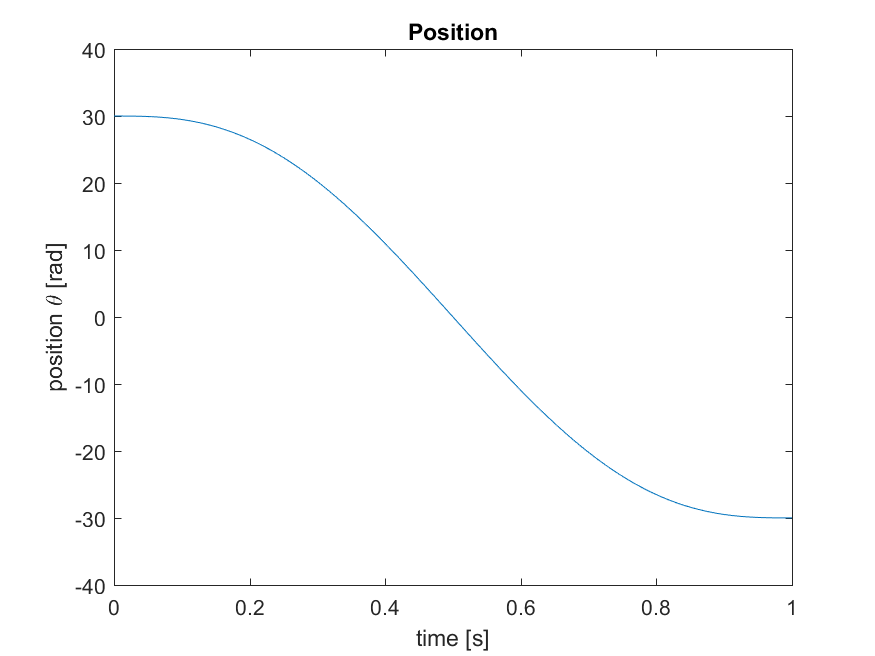
\includegraphics[width=\linewidth]{plot_position}
    \caption{Joint variable normal}
    \label{plot_position}
\end{subfigure}
\hfill
\begin{subfigure}{0.5\textwidth}
    \centering
    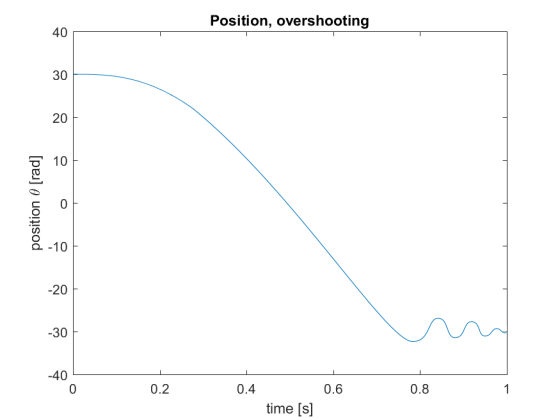
\includegraphics[width=\linewidth]{plot_position_over_edit}
    \caption{Overshooting the wanted joint position}
    \label{plot_position_over}
\end{subfigure}
\caption{Adjusting the joint angle correctly and with an overshoot}
\label{joint_position}
\end{figure}

Another issue arises when the suction cup has to press down on the package. The robot has to press down with sufficient force, but not too much as this could damage the package. Simple moment equations can be used to calculate this for a static situation, but in a situation where the package and/or the robot is moving inertial forces has to be accounted for when making these calculations.



\todo[inline]{
\textbf{Todo}

- the attempts of controlling a real robotic arm has provided mixed results, with a more robust framework for modelling dynamic behaviour and join limitations the system might be able to take these factors into account

- if not knowing the physical state of the robot and it's limitations, you might command the motors to perform tasks which goes beyond their limitation and may damage the motors, if knowing the dynamics that are in play in the robot and the limitations of the motors it will be possible to create control algorithms that prevent the motors from damaging itself
}

\section{Objective}

\todo[inline]{
\textbf{Todo}

- determine which physical parameters are important and influential to correctly control a robot, also determine if any properties does not have a significance that it is worth investing the time

- gather information and knowledge on how dynamics of a modern robot work

- develop a robust theoretical framework of the most important physical parameters

- find a good strategy for combining the current work that has been done in GeoMod and a robot model that incorporates the wanted physical properties and calculations

- perform an implementation of the new properties in the current model

- focus on serial link manipulators with fixed base, these are most the popular configuration. The framework can be expanded to undetermined ROV's at a later stage
}

\section{Approach}

\todo[inline]{
\textbf{Todo}

- Computer visualization of a robot and physical control are performed in two very different ways and use in some places very different math

- This provides to ways of tackling the problem, either with the computer visuals as a basis and implementing physical properties, or the other way around with the physical model as a framework

- As the final goal is to control real robots it would make sense to use the physical properties as a baseline

- On the other hand it seems like GeoMod has a focus on the computer graphics with OpenGL at it's core, this means that physical properties has to be derived from a framework that did not have this intention

- A solution could be to define a robot model with it's physics as it's baseline and at the same time making sure that the final solution would be possible to implement into GeoMod with as few compromises as possible.

- A good framework is one which will work for a broad spectrum of different configuration. It is therefore important to find a general solution which does not require any specific / hard coded parameters.
}